\documentclass[tikz]{standalone}
\usepackage{bm}
\usetikzlibrary{patterns}
\begin{document}
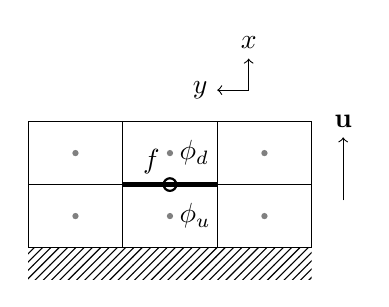
\begin{tikzpicture}[
  scale=0.4,
  cpnt/.style={fill=gray},
]

\fill [pattern=north east lines] (0,-1) rectangle (9,0);
\draw (0,0) rectangle (9,4);
\draw (3,0) -- (3,4);
\draw (6,0) -- (6,4);
\draw (0,2) -- (9,2);
\draw (0,4) -- (9,4);

\draw [->] (10,1.5) -- (10,3.5) node [above] {$\mathbf{u}$};
\draw [ultra thick] (3,2) -- (6,2);
\draw [thick] (4.5,2) circle [radius=0.2] node [anchor=south east] {$f$};

\path [cpnt] (1.5,1) circle [radius=0.1];
\path [cpnt] (4.5,1) circle [radius=0.1] node [right] {$\phi_u$};
\path [cpnt] (7.5,1) circle [radius=0.1];
\path [cpnt] (1.5,3) circle [radius=0.1];
\path [cpnt] (4.5,3) circle [radius=0.1] node [right] {$\phi_d$};
\path [cpnt] (7.5,3) circle [radius=0.1];

\draw [<->] (6,5) node [left] {$y$} -- (7,5) -- (7,6) node [above] {$x$};

\end{tikzpicture}
\end{document}
